%%%%%%%%%%%%%%%%%%%%%%%%%%%%%%%%%%%%%%%%%%%%%%%%%%%%%%%%%%%%%%%%%%%%%%
%%%%%%%%% Select one of the options, and comment the rest of them

%%%%%%%%%% Option 1:  to compile with pdflatex : parameter "t" - to align to the top
\documentclass[professionalfonts,t]{beamer}
%sans font?

%%%%%%%%%% Option 3: to create handout for print
%\documentclass[t,handout]{beamer}
%\usepackage{pgfpages}              % to put several slides on one page
%\pgfpagesuselayout{2 on 1}[a4paper, border shrink=5mm]             % 2 slides on 1 page
%\pgfpagesuselayout{4 on 1}[a4paper,landscape, border shrink=5mm]   % 4 slides on 1 page, and landscaped


%%%%%%%%%%%%%%%%%%%%%%%%%%%%%%%%%%%%%%%%%%%%%%%%%%%%%%%%%%%%%%%%%%%%
%%%%%%%%%%%%%% Select the Theme %%%%%%%%%%%%%%%%%%%%%%%%%%%%%%%%%%%
\usetheme{Dresden}     % OK
%\usetheme{Berlin}
%\usetheme{Bergen}      % NO
%\usetheme{Boadilla}    % NO
%\usetheme{Copenhagen}  % NO
%\usetheme{Hannover}    % NO
%\usetheme{Luebeck}     % NO
%\usetheme{Marburg}     % NO
%\usetheme{Pittsburgh}  % NO
%\usetheme{default}
%\usetheme{Singapore}   % OK
%\usetheme{boxes}
%\usecolortheme{structure}
%\usecolortheme{rose}
%\usecolortheme{beaver}


\definecolor{mymaroon}{cmyk}{0.0, 1.0, 1.0, 0.498}
\definecolor{myblue}{cmyk}{1.0, 1, 0, 0.5}
\definecolor{mygreen}{cmyk}{100, 0, 100, 50}
\setbeamercolor*{palette secondary}{use=structure,fg=white,bg=myblue}
\setbeamercolor*{palette tertiary}{use=structure,fg=white,bg=mymaroon}

%\usepackage{beamerthemesplit}              %
\beamertemplateballitem % fancy bullets and numbering

\setbeamertemplate{navigation symbols}{}   % suppress navigation symbols
\addtobeamertemplate{frametitle}{}{%
	\logo{../../images/IIT_logo}
	\iffalse
	
	\begin{tikzpicture}[remember picture,overlay]
	\node[anchor=center, yshift=-13pt, xshift=-5pt] at (current page.north) 
	{\includegraphics[height=1.1cm]{../images/Argonne_cmyk_black-eps-converted-to}\hspace{10cm}};
	
	\node[anchor=north east, yshift=3pt, xshift=0pt] at (current page.north east) 
	{\includegraphics[height=0.7cm]{../images/IIT_Logo_blk}};
	\end{tikzpicture}
    
     \fi
}
% other possibilities to include LOGO. it puts it in RLC

%
%\pgfdeclareimage[width=1cm]{logo}{../images/IIT_Logo}
%\logo{\pgfuseimage{logo}}


% load additional packages

\usepackage{xcolor}
\usepackage{graphicx}
\usepackage{amsmath}
\usepackage{amssymb}
\usepackage{amsthm}
\usepackage{graphicx}
\usepackage{url}
\usepackage{color}
\usepackage{booktabs} % Allows the use of \toprule, \midrule and \bottomrule in tables
\usepackage{pifont}% http://ctan.org/pkg/pifont
\usepackage{epstopdf}
\usepackage[export]{adjustbox}
\usepackage{tikz}
\usetikzlibrary{shapes.misc}
\usetikzlibrary{shapes,arrows,decorations.markings,shadows,positioning}

% Your Abbreviations
\newcommand\bE{{\mathbb{E}}}
\newcommand\bR{{\mathbb{R}}}
\newcommand\bH{{\mathbf{H}}}
% End abbreviations

\newcommand\Wider[2][3em]{%
	\makebox[\linewidth][c]{%
		\begin{minipage}{\dimexpr\textwidth+#1\relax}
			\raggedright#2
		\end{minipage}%
	}%\textbf{}
}

%%%%%%%%%%%%%%%%%%%%% to edit the main text below
%NOTES ON SOME TECHNICS
%%%% Box %%%%%%%%%%%%%%%%%%%%%%%%%%%%%%%%%%%%%%%%%%%%%%%
%{\fbox{ \parbox[t]{10cm}{ SOME TEXT }}}

%%% include a picture. The file should be with extention EPS, e.g. FILENAME.EPS
%\begin{figure}[h]
%\centering
%\includegraphics[width=.7\linewidth]{FILENAME}
%\caption{{\footnotesize PUT_CAPTION }}
%\end{figure}

%\subtitle{}
%\institute[ANL/IIT]{Argonne National Laboratory\\Illinois Institute of Technology}

\title[May 2018]{Preliminary TBA Beam Line}
\author[N.Neveu]{{\Large Nicole Neveu}}
\institute[ANL, IIT] % (optional, but mostly needed)
{   Illinois Institute of Technology \\
	Argonne National Laboratory \\
    \url{nneveu@anl.gov} 
}
% - Use the \inst command only if there are several affiliations.
% - Keep it simple, no one is interested in your street address.
\date{ \today \\
\includegraphics[width=3cm,keepaspectratio]{/home/nicole/Documents/presentations/logos/Argonne_cmyk_black}%
\hfill \hfill \hfill%
\includegraphics[width=4cm,keepaspectratio]{/home/nicole/Documents/presentations/logos/IIT_Logo_blk-eps-converted-to}%
}

%\date[IIT, April 2009]{
%           Space Charge 2017 \\ Oc 18, 2009  }



\begin{document}


\begin{frame}
  \titlepage
\end{frame}


\begin{frame}
	\frametitle{Outline}
	\tableofcontents
\end{frame}

\section{TBA Layout}
\begin{frame}
\frametitle{Introduction}
Premise: 
\begin{itemize}
	\item Consider hardware constraints
	\item Favor easy operating parameters
\end{itemize}

\vspace{0.5em}
TBA Requirements:
\begin{itemize}
	\item 100\% transmission 
	\begin{itemize}
		\item good beam size at structure
	\end{itemize}
	\item Reasonable bunch length at structure
	\begin{itemize}
		\item to maximize power generated
	\end{itemize}
\end{itemize}
	 
\end{frame}



%%%%%%%%%%%%%%%%%%%%%%%%%%%%%%%%%%%%%%%%%%%%%%%%%%%%%%%%%%%%%%%%%%%%%%%%%%%%%%%%


\begin{frame}
	\frametitle{TBA Bent Beam Layout}
	\begin{tikzpicture}[scale=\textwidth/22cm, text=black]
	%\begin{tikzpicture}[scale=0.5, text=black]
	\input{bentbeam.tex}
	\end{tikzpicture}
	
	\vspace{-1em}
	Mechanical considerations:
	\begin{itemize}
		\item 1m between kicker and septum
		\begin{itemize}
			\item for separation $\ge$ 50mm in septum. 
		\end{itemize}
		\item 1.8m between septum and dipole
		\begin{itemize}
			\item for separation $\ge$ 0.5m of beam lines.
		\end{itemize}
		\item 15cm between quads for easy installation. 
		\item 0.3m between quads and PETS for yag screen.  
	\end{itemize}
\end{frame}
%%%%%%%%%%%%%%%%%%%%%%%%%%%%%%%%%%%%%%%%%%%%%%%%%%%%%%%%%%%%%%%%%%%%%%%%%%%%%%%%
\iffalse
\section{Optimization}
\begin{frame}
\frametitle{TBA Optimization}
	\vspace{-0.75em}
	\begin{tikzpicture}[scale=\textwidth/26cm, text=black]
	%\begin{tikzpicture}[scale=0.5, text=black]
	\input{bentbeam.tex}
	\end{tikzpicture}
	%\caption{TBA beam line layout at the AWA. The arrow at the end of each line indicates what direction the beam is traveling.
		%PETS stands for Power Extraction and Transfer Structure, and ACC
		%stands for Accelerating structure. The subscript index on each structure refers to which stage the structures belong to, first or second stage. }

\vspace{-1em}
First round, 13 design variables:

Simplest, and worst case scenario (no phase control).

These variables are swept during optimization runs.
\begin{table}[hbt] 
	\centering
	\begin{tabular}{ l *{3}{c}}
		\toprule
		\textbf{Variable} & \textbf{Range} & \textbf{Unit} \\
		\midrule
		Buck Focusing Sol. &  $ 50 \le S_1 \le 440$ & amps \\
		Matching Solenoid & $ 350 \le S_2 \le 500$  & amps \\
		Phase of Gun & $-30 \le \phi_g \le 0.0$  & degrees \\
		Laser FWHM & $1.5 \le T \le $10  & ps \\
		Quads$_{1-9}$ & $-8 \le Q_n \le 8$  & T/m \\
		\bottomrule	
	\end{tabular}

	
\end{table}
\end{frame}
%%%%%%%%%%%%%%%%%%%%%%%%%%%%%%%%%%%%%%%%%%%%%%%%%%%%%%%%%%%%%%%%%%%%%%%%%%%%%%%%
\begin{frame}
\frametitle{TBA Location(s) of Interest}

\begin{minipage}{0.6\textwidth}
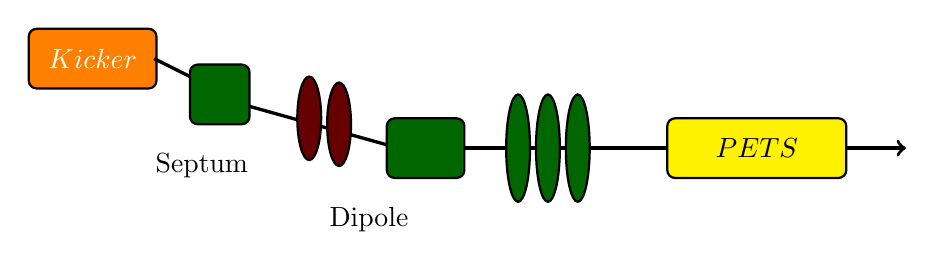
\begin{tikzpicture}[scale=\textwidth/16cm]
\def \gunleft {-1.0}
\def \gunright {0.3}
\def \loneright {1.0}
\def \ltworight {2.0}
\def \lthreeright {3.0}
\def \lfourright {4.0}
\def \lfiveright {5.0}
\def \lsixright {-6}
\def \quadone {7.3}
\def \quadfour{5}
%Septum
\node[] at (0.2,-0.8) {Septum};
\draw[fill=black!60!green,  thick, rounded corners =0.1cm] (0.0,0.9)rectangle ({1},-0.1) node[pos=.5, white] {};

%Line between septum and dipole
\draw[very thick] (1,0.2) -- (3.5,-0.5);

%Quads between septum and dipole
\draw[fill=black!60!red,  thick] (\loneright+1, 0.0) ellipse (0.2cm and 0.7cm);
\draw[fill=black!60!red,  thick] (\loneright+1.5, -0.1) ellipse (0.2cm and 0.7cm);

%Line between dipole and quads
\draw[very thick, ->] (3.6,-0.5) -- (12,-0.5);

%Dipole
\node[] at (3,-1.7) {Dipole};
\draw[fill=black!60!green, thick, rounded corners =0.1cm] (3.3,0.0)rectangle ({4.6},-1.0) node[pos=.5, white] {};


%Second set of quads
\draw[fill=black!60!green,  thick] (\quadfour+0.5, -0.50) ellipse (0.2cm and 0.9cm);
\draw[fill=black!60!green,  thick] (\quadfour+1.0, -0.50) ellipse (0.2cm and 0.9cm);
\draw[fill=black!60!green,  thick] (\quadfour+1.5, -0.50) ellipse (0.2cm and 0.9cm);

%Kicker 
\draw[fill=orange,  thick, rounded corners =0.1cm] (\lsixright+3.3,0.5)rectangle ({\lsixright+0.84+4.6},1.5) node[pos=.5, white] {$Kicker$};

%Line between kicker and septum
\draw[very thick] (-0.6,1) -- (0,0.7);

%PETS 
\draw[fill=yellow,  thick, rounded corners =0.1cm] (\lsixright+14,0.0)rectangle ({\lsixright+17},-1.0) node[pos=.5, black] {$PETS$};
\end{tikzpicture}	
\end{minipage}
\begin{minipage}{0.35\textwidth}
	Tried two scenarios: with and without quads between septum and dipole.
\end{minipage}

\vspace{1em}
\begin{minipage}{0.55\textwidth}
	\begin{table}[hbt] 
	\centering
	\begin{tabular}{ l *{3}{c}}
		\toprule
		\textbf{Description} & \textbf{Location} & \textbf{Length} & \textbf{Aperture}\\
		\midrule
		Entrance of Kicker, 	$ z_k$ 		& 16.5 m & 1 m   & 40 mm\\
		Entrance of Septum, 	$ z_s$  	& 18.5 m & 0.2 m & 25 mm\\
		Center of Doublet, 		$ z_{q1}$	& 19.5 m & -- 	 & 50 mm\\
		Entrance of Dipole, 	$ z_d$  	& 20.5 m & 0.2 m & 50 mm\\
		Center of Triplet,		$ z_{q2}$	& 21.2 m & --    & 50 mm\\
		Entrance of PETS, $z_{pets1}$  & 21.8 m & 0.4 m 	 & 17.6 mm\\
		After PETS, 			$z_{pets2}$ & 22.5 m &  --   & 17.6 mm\\
		\bottomrule	
	\end{tabular}	
\end{table}
\end{minipage}
\end{frame}
%%%%%%%%%%%%%%%%%%%%%%%%%%%%%%%%%%%%%%%%%%%%%%%%%%%%%%%%%%%%%%%%%%%%%%%%%%%%%%%%
\begin{frame}
	\frametitle{Optimization Objectives}
	Objectives are beam parameters the simulation tries to minimize.
	These points are picked to improve beam parameters at key locations, 
	i.e. the PETS structure.
	
	\vspace{1em}
\begin{minipage}{0.45\textwidth}
		\begin{table}[hbt] 
		\centering
		\begin{tabular}{ l *{3}{c}}
			\toprule
			\textbf{Variable} &  \textbf{Unit} \\
			\midrule
			$\sigma_z$ 		& mm \\
			$\sigma_{x}$ 	& mm \\
			$\sigma_y$ 		& mm \\
			$\sigma_{px}$ 	& mm-mrad \\
			$\sigma_{py}$ 	& mm-mrad \\
			$dE$			& MeV\\
			\bottomrule	
		\end{tabular}	
	\end{table}
\end{minipage}
\begin{minipage}{0.45\textwidth}
	\begin{itemize}
		\item 3 optimized locations ($z_k$, $z_s$, $z_d$)
		\item 18 Objectives
		\item 10 variables 
		\item 6 Constraints
	\end{itemize}
\end{minipage}
\centering
Note, these take an extremely large time to simulate (order days).
\end{frame}
\fi
%%%%%%%%%%%%%%%%%%%%%%%%%%%%%%%%%%%%%%%%%%%%%%%%%%%%%%%%%%%%%%%%%%%%%%%%%%%%%%%%
\begin{frame}
\frametitle{PETS}
\begin{itemize}
	\item Reminder: form factor and bunch length are related. 
	\item Will continue to try to reduce bunch length
\end{itemize}

\begin{minipage}{0.49\textwidth}
\includegraphics[width=\textwidth]{{/home/nicole/Documents/awa-tba/pareto_stat_plots/zrms-optLinac-40nC_KQ3=3.2_KQ5=-1.25_KQ6=-0.25_KQ7=0_KQ8=0}.pdf}
\end{minipage}
\begin{minipage}{0.49\textwidth}

\centering
\includegraphics[width=\textwidth]{/home/nicole/Documents/thesis_code/formfactorsqrd}
\end{minipage}
\end{frame}
%%%%%%%%%%%%%%%%%%%%%%%%%%%%%%%%%%%%%%%%%%%%%%%%%%%%%%%%%%%%%%%%%%%%%%%%%%%%%%%%
\section{Results}
\begin{frame}
\vspace{-1em }

\frametitle{Scenario 1: Last Triplet off}
\vspace{-1em}

\hfill	\small{\begin{itemize}
		\item Symmetric beam not necessary, if transmission is good.
		\item PETS aperture = 17.6 mm
		\item Need to adjust matching and quads.
\end{itemize}}

\vspace{2em}

\begin{minipage}{0.45\textwidth}

\centering	
2D Field Maps only

\includegraphics[width=\textwidth]{{/home/nicole/Documents/awa-tba/pareto_stat_plots/xyrms-optLinac-40nC_KQ3=3.2_KQ5=-1.25_KQ6=-0.25_KQ7=0_KQ8=0}.pdf}	
\end{minipage}
\begin{minipage}{0.45\textwidth}
	
	\centering
	3D Maps and CSR included
	
\includegraphics[width=\textwidth]{{/home/nicole/Documents/awa-tba/pareto_stat_plots/xyrms-csr_fields}.pdf}		
\end{minipage}
\end{frame}
%%%%%%%%%%%%%%%%%%%%%%%%%%%%%%%%%%%%%%%%%%%%%%%%%%%%%%%%%%%%%%%%%%%%%%%%%%%%%%%%
\begin{frame}
\frametitle{Scenario 1: Last Triplet off}
\vspace{-1em}

\hfill	\small{\begin{itemize}
		\item 3D Maps and CSR included
		\item Difference in energy due to CSR = 0.2 MeV
\end{itemize}}

\vspace{2em}

\begin{minipage}{0.45\textwidth}
	
	\centering	
	
	Energy 65 MeV
	\includegraphics[width=\textwidth]{{/home/nicole/Documents/awa-tba/pareto_stat_plots/energy-csr_fields}.pdf}	
\end{minipage}
\begin{minipage}{0.45\textwidth}
	
	\centering
	Max beam size and pipe
	
	\includegraphics[width=\textwidth]{{/home/nicole/Documents/awa-tba/pareto_stat_plots/xy-max-min-csr_fields}.pdf}		
\end{minipage}
\end{frame}
%%%%%%%%%%%%%%%%%%%%%%%%%%%%%%%%%%%%%%%%%%%%%%%%%%%%%%%%%%%%%%%%%%%%%%%%%%%%%%%%
\begin{frame}
\frametitle{Scenario 1: Lower Matching}
\begin{itemize}
	\item Can run 3D optimization of quads, with narrow boundaries
\end{itemize}

\centering
	M = 220 \hspace{5em} M=225 \hspace{5em} M=230

	\includegraphics[width=0.3\textwidth]{{/home/nicole/Documents/awa-tba/pareto_stat_plots/xyrms-optLinac-40nC_KQ3=3.2_IM=220}.pdf}%	
	\includegraphics[width=0.3\textwidth]{{/home/nicole/Documents/awa-tba/pareto_stat_plots/xyrms-optLinac-40nC_KQ3=3.2_IM=225}.pdf}%	
	\includegraphics[width=0.3\textwidth]{{/home/nicole/Documents/awa-tba/pareto_stat_plots/xyrms-optLinac-40nC_KQ3=3.2_IM=230}.pdf} \\%
	\includegraphics[width=0.3\textwidth]{{/home/nicole/Documents/awa-tba/pareto_stat_plots/xy-max-min-optLinac-40nC_KQ3=3.2_IM=220}.pdf}%	
	\includegraphics[width=0.3\textwidth]{{/home/nicole/Documents/awa-tba/pareto_stat_plots/xy-max-min-optLinac-40nC_KQ3=3.2_IM=225}.pdf}%	
	\includegraphics[width=0.3\textwidth]{{/home/nicole/Documents/awa-tba/pareto_stat_plots/xy-max-min-optLinac-40nC_KQ3=3.2_IM=230}.pdf}%

\end{frame}
%%%%%%%%%%%%%%%%%%%%%%%%%%%%%%%%%%%%%%%%%%%%%%%%%%%%%%%%%%%%%%%%%%%%%%%%%%%%%%%%
\begin{frame}
	\frametitle{Scenario 1: cont..}
\Wider{
	
	\begin{minipage}{0.6\textwidth}
		Gun Settings:
		
	\begin{table}[hbt] 
		\centering
		\begin{tabular}{ l *{3}{c}}
			\toprule
			\textbf{Variable} &  \textbf{Value} & \textbf{Unit} \\
			\midrule
			Gun Phase		  &-20& degrees \\
			FWHM		 	  &10& ps \\
			Laser Radius	  &9.0& mm \\
			Matching Solenoid &250& amps \\
			Buck Focusing     &500& amps \\
			\bottomrule	
		\end{tabular}	
	\end{table}	
	\end{minipage}
		\begin{minipage}{0.35\textwidth}
		Quad Settings:
		\begin{table}[hbt] 
			\centering
			\begin{tabular}{ l *{3}{c}}
				\toprule
				\textbf{Variable} &  \textbf{Value} & \textbf{Unit} \\
				\midrule
				Q1	  &0.0  & amps \\
				Q2 	  &-1.7 & amps \\
				Q3	  &3.3  & amps \\
				Q4    &-1.7 & amps \\
				Q5    &-1.25& amps \\
				Q6	  &-0.25& amps \\
				Q7	  & 0 & amps \\
				Q8    & 0 & amps \\
				Q9    & 0 & amps \\
				\bottomrule	
			\end{tabular}	
		\end{table}	
	\end{minipage}
}
\end{frame}



\iffalse
\begin{frame}
\frametitle{Sensitivity Analysis}
\vspace{-0.5em}
Mismatch in energy, matching solenoid, or \textbf{quads} could cause problems. 
Beam results are weakened if these do not match.
\centering
\includegraphics[width=0.8\textwidth]{/home/nicole/Documents/surrogatemodels/ml-ws-poster/awa-medium-o4/sensresults.pdf}
\end{frame}
\fi


\section{Recent Energy Measurements}
\begin{frame}
\frametitle{Energy Measurements: 06/27}
	\begin{itemize}
		\item Max total energy $\approx$ 62 MeV
		\item Min total energy $\approx$ 58 MeV
		\item Gun, L1, L2 $\approx$ 25 MeV
		\item Gun, L3, L5 $\approx$ 24 MeV
		\item Gun, L4, L6 $\approx$ 22 MeV
		\item Measurments pre-2018
		\begin{itemize}
			\item Mean total energy $\approx$ 65 MeV (low charge)
			\item Mean total energy $\approx$ 63 MeV (high charge)
			\item Gun, L1, L2 $\approx$ 26.5 MeV
			\item Gun, L1, L2, L3, L5 $\approx$ 46 MeV
		\end{itemize}
	\end{itemize}
	
	I will compare this with dipole downstream from Friday 07/06.
	
	I suggest a log of careful energy measurements for better statistics.
	
\end{frame}



%%%%%%%%%%%%%%%%%%%%%%%%%%%%%%%%%%%%%%%%%%%%%%%%%%%%%%%%%%%%%%%%%%%%%%%%%%%%%%%%
\begin{frame}
	\frametitle{Summary}
	\begin{itemize}
		\item Future simulation steps:
		\begin{itemize}
			\item 3D optimization of quad settings

		\end{itemize}
		\item Match simulations to machine - critical step for TBA
		\item Reminder: Near term proposed beam studies don't require more hardware
		\begin{itemize}
			\item Phase control test
			\item Quad beam size comparison
			\item Kicker voltage scan
			\item More energy measurements
			\item Bunch length and emittance
		\end{itemize}
		\item Beam studies needed to ensure success of TBA.
		
	\end{itemize}
\end{frame}


%%%%%%%%%%%%%%%%%%%%%%%%%%%%%%%%%%%%%%%%%%%%%%%%%%%%%%%%%%%%%%%%%%%%%%%%%%%%%%%%
\section{Backup}
\iftrue
\begin{frame}
	\frametitle{Backup Slides}
\end{frame}



\begin{frame}
\frametitle{Energy Spread and Emittance}
\vspace{1em}

Need to reduce energy spread with phase control

\vspace{1em}

\begin{minipage}{\textwidth}
	
	\centering
	\includegraphics[width=0.45\textwidth]{{/home/nicole/Documents/awa-tba/pareto_stat_plots/dE-csr_fields}.pdf}\includegraphics[width=0.45\textwidth]{{/home/nicole/Documents/awa-tba/pareto_stat_plots/emit-csr_fields}.pdf}
\end{minipage}
\end{frame}




\fi

\begin{frame}
\vspace{-1em}

\frametitle{Scenario 2: Last triplet on}
\vspace{-1em}

\hfill	\small{\begin{itemize}
		\item Symmetric beam not necessary, if transmission is good.
		\item PETS aperture = 17.6 mm
\end{itemize}}
\centering
\includegraphics[width=0.75\textwidth]{{/home/nicole/Documents/awa-tba/pareto_stat_plots/xyrms-optLinac-40nC_KQ3=3.3_KQ5=-1.25_KQ6=-0.25_KQ7=0.5_KQ8=0}.pdf}
\end{frame}






\end{document}
















